\chapter{ML with TensorFlow}

Overview

\section{Introduction}

\section{Artificial Neural Networks}

\subsection{History}

\textcolor{blue}{McCullock and Pitts -- nerve cell as a simple logic gate with binary outputs.  Where multiple input signals are accumulated and if they exceed a certain threshold an output signal is generated}

\textcolor{blue}{Frank Rosenblatt -- the perceptron: an algorithm that would learn the optimal weight coefficients to the input features in order to determine whether an output signal should be produced. The early activation function \textcolor{red}{See more in local ref?} was a simple unit step function.}

\textcolor{blue}{Adaline (\textbf{ADA}ptive \textbf{LI}near \textbf{NE}uron) -- rather than the weights being updated based on a unit step function like the perceptron, the weights are updated based on a linear activation function. A continuous output value (rather than discrete) is used to compute the model error and update the weights.}

\textcolor{blue}{Linear activation function is used for weight updates but a unit step function can still be used to predict the class labels.\textcolor{red}{TODO: figure showing this}}

\section{Convolutional Neural Networks}

\section{Recurrent Neural Networks}

\section{Weight Initialization}

%%%%% activation functions
\subsection{Activation Functions}

\textcolor{blue}{Activation functions are XXXXXXXX}

\subsubsection{Why Non-linear}

\textcolor{blue}{Non-linear is necessary XXXXXXXXXX}

\subsubsection{Advancements}

\textcolor{green}{TODO: From step function to ?selu}

\subsubsection{Popular Activation Functions}

\textcolor{blue}{Activation functions can be grouped into two main categories -- smooth and not smooth. Smooth activation functions (such as sigmoid) are differentiable at every point along the function where as the other activation functions are not differentiable at every location (relu).}

% history
%differentiable everywhere, monotonic, and smooth.

\textcolor{blue}{linear (see above), }
	
\textcolor{blue}{tanh and sigmoid, (better because non-linear). however would saturate}

\textcolor{blue}{ReLu, better because \textcolor{red}{help prevent saturation}, but still have problems \textcolor{red}{can "die" at 0.} }

\textcolor{blue}{ELU fuctions. they prevent the "dying" problem by being \textcolor{red}{non-zero} but their main drawback is that they are more computationally expensive due to the calculation of the exponent.}

\paragraph{Smooth Non-linear}

\subparagraph{Sigmoid}

\textcolor{blue}{The sigmoid\index{sigmoid} activation function.}

\textcolor{blue}{calibrated probability estimate}


% {{{act_smooth_sigmoid}}}
\begin{figure}
\centering
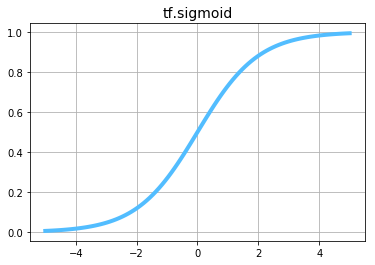
\includegraphics[width=0.65\textwidth]{./sync_imgs/act/smooth/sigmoid.png}
\label{fig:act_smooth_sigmoid}
\end{figure}

% {{{act_smooth_tangent}}}
\begin{figure}
\centering
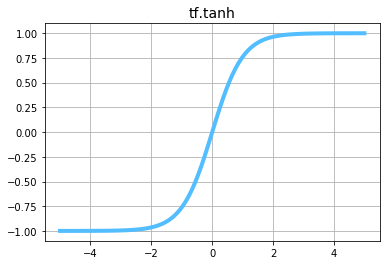
\includegraphics[width=0.65\textwidth]{./sync_imgs/act/smooth/tangent.png}
\label{fig:act_smooth_tangent}
\end{figure}

\subparagraph{ELU}

\textcolor{blue}{\textcolor{red}{CITE}. Smooth, monotonic, and non-zero in the negative portion of the input. The main drawback is that they are more computationally expensive (due to calculating the exponential)}


\begin{equation}
{
	ELU = f(x) = \left\{
	\begin{array}{ll}
	\alpha(e^x - 1) x & \quad $for$ \ x < 0 \\
	x & \quad $for$ \ x \ge 0
	\end{array}
	\right.
}
\label{eq:act_elu_def}
\end{equation}


% {{{act_smooth_elu}}}
\begin{figure}
\centering
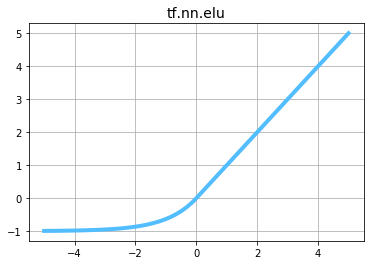
\includegraphics[width=0.65\textwidth]{./sync_imgs/act/smooth/elu.png}
\label{fig:act_smooth_elu}
\end{figure}

% {{{act_smooth_selu}}}
\begin{figure}
\centering
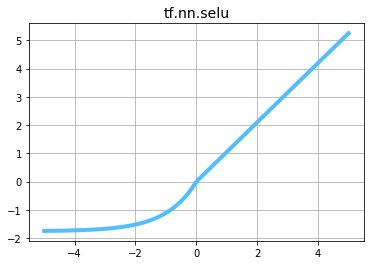
\includegraphics[width=0.65\textwidth]{./sync_imgs/act/smooth/selu.png}
\label{fig:act_smooth_selu}
\end{figure}


\subparagraph{Softplus}

\textcolor{blue}{continuous and differentiable at zero. However, due to the natural log and exponential function, there is added computation compared to th ReLU.}

% typcially discouraged in practice since ReLU achieves similar results and is less computationally expensive

\begin{equation}
{
	Softplus = f(x) = \ln{(1+e^x)}
}
\label{eq:act_softplus_def}
\end{equation}


% {{{act_smooth_softplus}}}
\begin{figure}
\centering
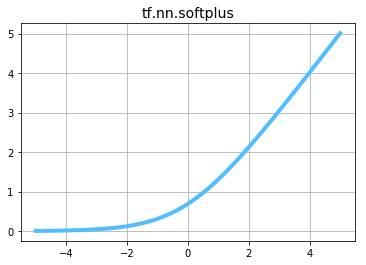
\includegraphics[width=0.65\textwidth]{./sync_imgs/act/smooth/softplus.png}
\label{fig:act_smooth_softplus}
\end{figure}

% {{{act_smooth_softsign}}}
\begin{figure}
\centering
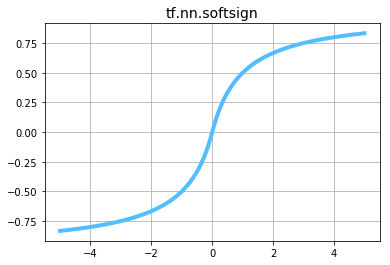
\includegraphics[width=0.65\textwidth]{./sync_imgs/act/smooth/softsign.png}
\label{fig:act_smooth_softsign}
\end{figure}


\paragraph{Not Smooth Non-linear}

\subparagraph{ReLU}

\begin{equation}
{
	ReLU = f(x) = \left\{
	\begin{array}{ll}
	0 & \quad $for$ \ x < 0 \\
	x & \quad $for$ \ x \ge 0
	\end{array}
	\right.
}
\label{eq:act_relu_def}
\end{equation}

% {{{act_notsmooth_relu}}}
\begin{figure}
\centering
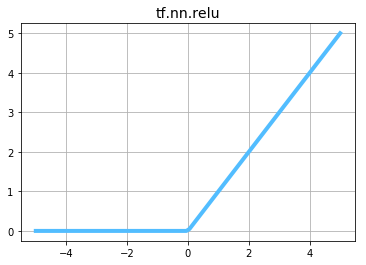
\includegraphics[width=0.65\textwidth]{./sync_imgs/act/notsmooth/relu.png}
\label{fig:act_notsmooth_relu}
\end{figure}

\subparagraph{Leaky ReLU}

\textcolor{blue}{The Leaky ReLU (Eq~\ref{eq:act_leaky_relu_def}) was designed in attempt to address the dying ReLU issue \textcolor{red}{CITE}. Rather than simply outputting a zero in the negative range, the Leaky ReLU will will have a small non-zero slope (user specified) -- allowing weight updating and training to continue.}

\textcolor{green}{TODO: randomized Leaky ReLU \textcolor{red}{cite} --- $\alpha$ (from PReLU) is sampled from a uniform distribution randomly. The net-effect could be considered similar to drop out since, technically, there is a different network for each value of $\alpha$, resulting in an ensemble of sorts. At test time, the values for $\alpha$ are averaged.}

\begin{equ}[!ht]
	\begin{equation}
	{
		Leaky ReLU = f(x) = \left\{
		\begin{array}{ll}
		N x & \quad $for$ \ x < 0 \\
		x & \quad $for$ \ x \ge 0
		\end{array}
		\right.
	}
	\label{eq:act_leaky_relu_def}
	\end{equation}
\caption{where $N$ is a constant. $N$ is typically set to 0.01}
\end{equ}

% {{{act_notsmooth_leakyrelu}}}
\begin{figure}
\centering
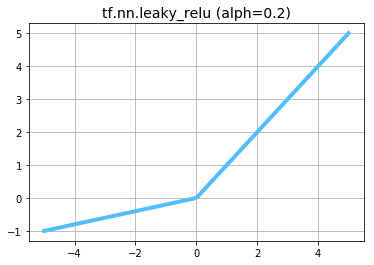
\includegraphics[width=0.65\textwidth]{./sync_imgs/act/notsmooth/leakyrelu.png}
\label{fig:act_notsmooth_leakyrelu}
\end{figure}

\subparagraph{ReLU6}

\textcolor{blue}{In general, this function is referred to as a {ReLUN}\index{ReLUN} function, where $N$ is some constant. However, in practice, $6$, was determined to be the optimal value.\textcolor{red}{CITE}. \textcolor{red}{This capped value, may help learn the sparse values sooner.} By having the upper limit bounded, the prepare the network for a fixed point precision for inference --- if the upper limit is unbounded, then you may loose too many bits to \textcolor{red}{Q} portion of the fixed point number.}
		

\textcolor{blue}{Similar to the ReLU fuction, only the output is capped to six in the positive domain.}

\begin{equation}
{
	ReLU6 = f(x) = min{(max{(0,x)},6)}
}
\label{eq:act_ReLU6_def}
\end{equation}

% {{{act_notsmooth_relu6}}}
\begin{figure}
\centering
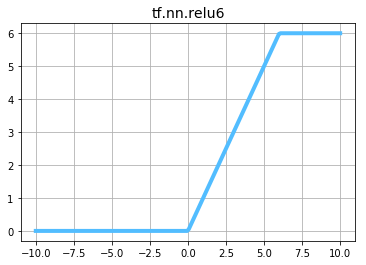
\includegraphics[width=0.65\textwidth]{./sync_imgs/act/notsmooth/relu6.png}
\label{fig:act_notsmooth_relu6}
\end{figure}

\subparagraph{PReLU}

\begin{equ}[!ht]
	\begin{equation}
	{
	PReLU = f(x) = \left\{
		\begin{array}{ll}
			\alpha x & \quad $for$ \ x < 0 \\
			x & \quad $for$ \ x \ge 0
		\end{array}
		\right.
	}
	\label{eq:act_prelu_def}
	\end{equation}
\caption{where $\alpha$ is a parameterized --- a learned parameter from training.}
\end{equ}

\textcolor{blue}{$\alpha$, rather than being hard coded, is determined during training by the data. The logic being that the value would be more optimal than we could set \textcolor{red}{CITE}}

% {{{act_notsmooth_prelu}}}
\begin{figure}
\centering
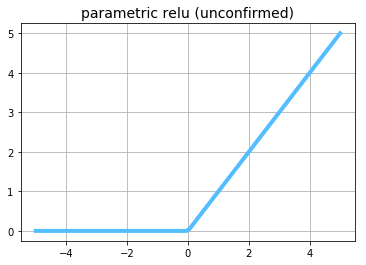
\includegraphics[width=0.65\textwidth]{./sync_imgs/act/notsmooth/prelu.png}
\label{fig:act_notsmooth_prelu}
\end{figure}



%%%%% Optimizers
\subsection{Optimizers}

\textcolor{blue}{Estimate the values of the model's parameters that minimize the value of the cost function}

\textcolor{blue}{"turning a loss function into a search strategy"}

\subsubsection{Gradient Descent}

\textcolor{blue}{Gradient Descent --- overview --- optimization algorithm that can be used to estimate the local minimum of a function}

\textcolor{blue}{Iteratively updates the model parameters by calculating the partial derivatives of the cost function at each step during training}

\textcolor{blue}{Gradient descent is only guaranteed to find the local minimum of the cost function.}

\textcolor{blue}{simultaneous update.}


\paragraph{Batch Gradient Descent}

\textcolor{blue}{batch gradient descent --- taking a step (update the weights) opposite (down) the gradient calculated from the entire training set}

\textcolor{blue}{Batch gradient descent is deterministic --- will produce the same paramter values if the same dataset is used multiple times.}


\paragraph{Stochastic Gradient Descent}

\textcolor{blue}{Stochastic Gradient Descent (sometimes called iterative or on-line gradient descent) --- rather than update the weights based on the sum of the accumulated errors, the weights are updated for each training sample}

\textcolor{blue}{Stochastic gradient descent is deterministic --- may produce the different parameter values if the same dataset is used multiple times. May not minimize the cost function as well as gradient descent but the approximation is often ``close enough''.}


\paragraph{Mini-batch Gradient Descent}

\textcolor{blue}{mini-batch gradient descent --- compromise between batch and stochastic gradient descent where the gradient is calculated over a batch of training data}

\textcolor{blue}{Since the gradient is calculated on a single example, the error surface will appear noisier than if it was calculated over a batch or the entire training set.}

\textcolor{blue}{When using stochastic gradient descent, it is important to shuffle the data after each epoch.}


% when looking at specific optimizers, http://ruder.io/optimizing-gradient-descent/ was a useful resource

\subsection{Improved Optimizers}

\textcolor{blue}{Some of the common optimizers are listed below. Additional optimizers are discussed in \textcolor{red}{local ref?}}

\subsubsection{Momentum}

\textcolor{blue}{Momentum~\cite{qian1999momentum}, will reduce the learning rate when the gradient is small}

\subsubsection{RMSProp}

\subsubsection{Nesterov}

\textcolor{blue}{Nesterov accelerated gradient (NAG)}

\subsubsection{Adam}

\textcolor{blue}{Adaptive Moment Estimation (Adam)~\cite{kingma2014adam}}


%%%%%%%%%%%%%%%%%%%%%%%%%%%%%%%%%%%%%%%%%%%%%%%%%%%%%%%%%%%%%%%%%%%%%%%%%%%%%%%%%%%%%%
%%%%%% TODO: Cut off -- these optimizers will be moved to another location (research?)
%%%%%%%%%%%%%%%%%%%%%%%%%%%%%%%%%%%%%%%%%%%%%%%%%%%%%%%%%%%%%%%%%%%%%%%%%%%%%%%%%%%%%%

\subsubsection{Nadam}

\textcolor{blue}{Nadam (Nesterov-accelerated Adaptive Moment Estimation)~\cite{dozat2016incorporating}}

\subsubsection{AdaGrad}

\textcolor{blue}{Adagrad~\cite{duchi2011adaptive}, will assign frequently occurring features low learning rates}

\subsubsection{AdaDelta}

\textcolor{blue}{Adadelta~\cite{zeiler2012adadelta}, expands on AdaGrad by avoiding reducing the learning rate to zero.}

\subsubsection{AdaMax}

\subsubsection{Ftrl}

\textcolor{blue}{``follow the regularized leader'', \textcolor{red}{CITE}, \textcolor{red}{works well on wide modes?}}








\section{Hyperparameters}

\subsection{Training Related}

\subsubsection{Learning Rate}

\paragraph{Too High vs Too Low}

\textcolor{blue}{TODO: figure showing a convex cost function and the result of a learning rate being too high (overshoot, diverge) and too small (local minima)}

\subsubsection{Batch Size}

\subsubsection{Number of Training Iterations}

\subsubsection{Momentum}

\subsubsection{Weight Update}

\textcolor{red}{SGD, CG, L-BFGS, more complex more hyper-parameters}

\subsubsection{Stopping Criteria}

\subsection{Model Related}

\subsubsection{Architecture}

\subsubsection{Weight Initialization}

\subsubsection{Weight-decay}

L1

L2

\subsubsection{Drop-out}

\section{Hyper-parameter optimization}

\textcolor{blue}{OVERVIEW}

\subsubsection{Coordinate Descent}

All hyper-parameters remain fixed, except for the hyper-parameter of interest. The hyper-parameter of interest is then adjusted such that the validation error is minimized.

\subsubsection{Grid Search}

\textcolor{green}{TODO: grid search explanation}

\subsubsection{Random Search}

\textcolor{green}{TODO: random search explanation}

\subsubsection{Grid vs Random Search}

\textcolor{green}{TODO: grid vs random search figure}

\subsubsection{Automated / Model-based Methods}


\section{Regularization}

\subsection{Why Regularization}

\subsection{Types of Regularization}

\subsubsection{Regularization Methods and Implementations}

\paragraph{L2 Regularization}

\paragraph{L1 Regularization}

\section{Image Augmentation}

\section{Serving}

\section{TensorBoard}

\section{Estimators}

\section{Metrics}

\section{Eager}

\section{Model Persistence}

